%% ============================================================
%%  SUSTENTACIÓN — autoTUG / TRL 6
%%  John Sebastian Chamorro Narváez
%%  Universidad del Valle — Ingeniería Electrónica, 2025
%% ============================================================
\documentclass[10pt,aspectratio=169]{beamer}

\usepackage[spanish]{babel}
\usepackage[utf8]{inputenc}
\usepackage{graphicx}
\usepackage{booktabs}
\usepackage{amsmath}
\usepackage{tikz}
\usetikzlibrary{arrows.meta,positioning,shapes.geometric,calc}
\usepackage{tabularx}
\usepackage{xcolor}
\usepackage{colortbl}
\usepackage{multirow}
\usepackage{subcaption}

% ========= Colores Universidad del Valle =========
\definecolor{uvblue}{RGB}{0,73,144}
\definecolor{uvgold}{RGB}{248,172,0}
\definecolor{uvdark}{RGB}{0,45,90}
\definecolor{lightblue}{RGB}{220,235,252}
\definecolor{lightgold}{RGB}{255,243,204}

% ========= Tema =========
\usetheme{Madrid}
\setbeamercolor{palette primary}{bg=uvblue,fg=white}
\setbeamercolor{palette secondary}{bg=uvblue!85!black,fg=white}
\setbeamercolor{palette tertiary}{bg=uvblue!65!black,fg=white}
\setbeamercolor{palette quaternary}{bg=uvblue,fg=white}
\setbeamercolor{frametitle}{bg=uvblue,fg=white}
\setbeamercolor{title}{fg=white}
\setbeamercolor{titlelike}{bg=uvblue,fg=white}
\setbeamercolor{block title}{bg=uvblue,fg=white}
\setbeamercolor{block body}{bg=lightblue}
\setbeamercolor{block title alerted}{bg=red!70!black,fg=white}
\setbeamercolor{block body alerted}{bg=red!8}
\setbeamercolor{alerted text}{fg=uvgold!80!black}
\setbeamercolor{structure}{fg=uvblue}
\setbeamercolor{itemize item}{fg=uvblue}
\setbeamercolor{itemize subitem}{fg=uvblue!70}
\setbeamercolor{enumerate item}{fg=uvblue}
\setbeamerfont{frametitle}{size=\large,series=\bfseries}
\setbeamerfont{block title}{series=\bfseries}

% ========= TikZ estilos =========
\tikzset{
  sblock/.style={
    rectangle, draw=uvblue, fill=lightblue, rounded corners=3pt,
    text width=3.0cm, align=center, minimum height=0.75cm, font=\small
  },
  sarrow/.style={draw=uvblue, -{Latex[length=2.5mm]}, thick}
}

% ========= Datos de la presentación =========
\title[autoTUG --- TRL~6]{%
  Aplicación para la Monitorización de la Prueba\\[2pt]
  \textit{Timed Up and Go} con Teléfono Inteligente,\\[2pt]
  Gestión de Información en la Nube y TRL~6}
\subtitle{Sustentación de Trabajo de Grado\\Ingeniería Electrónica}
\author[Chamorro Narváez, J.S.]{John Sebastian Chamorro Narváez}
\institute[Univalle]{%
  Escuela de Ingeniería Eléctrica y Electrónica\\
  Universidad del Valle\\[0.4em]
  {\small Directores: Dr.-Ing. Esteban Rosero
         \quad J.M. Ramírez Scarpetta, Ph.D.}\\
  {\small Grupo de Investigación en Control Industrial (GICI)}%
}
\date{Santiago de Cali, 2025}

% ========= Secciones para la barra de navegación =========
\AtBeginSection[]{%
  \begin{frame}[plain]
    \vfill
    \centering
    {\usebeamerfont{title}\usebeamercolor[fg]{frametitle}\insertsectionhead}
    \vfill
  \end{frame}%
}

% ============================================================
\begin{document}

% -------- DIAPOSITIVA 1: PORTADA --------
\begin{frame}[plain]
  \begin{columns}[c]
    \column{0.76\textwidth}
      \titlepage
    \column{0.22\textwidth}
      \centering
      
\includegraphics[width=\linewidth]{Images/LogoUnivalle.jpg}
  \end{columns}
\end{frame}

% -------- DIAPOSITIVA 2: CONTENIDO --------
\begin{frame}{Contenido}
  \tableofcontents
\end{frame}

% ============================================================
\section{Contexto y Motivación}

% -------- DIAPOSITIVA 3: LA PRUEBA TUG --------
\begin{frame}{Prueba \textit{Timed Up and Go} (TUG)}
  \begin{columns}[c]
    \column{0.50\textwidth}
      \begin{block}{¿Qué es?}
        Prueba funcional estándar para evaluar movilidad básica:\\[0.4em]
        \textbf{Levantarse} $\to$ Caminar 3\,m $\to$ \textbf{Girar 180°}
        $\to$ Regresar $\to$ \textbf{Sentarse}
      \end{block}
      \vspace{0.5em}
      \begin{itemize}
        \item Ampliamente usado en clínica para adultos mayores
        \item Versión clásica: \textbf{solo el tiempo total}
        \item iTUG extrae \alert{variables temporales y cinemáticas por subfase}:
              tiempos, aceleraciones, rotación, flexión/extensión del tronco
      \end{itemize}
    \column{0.48\textwidth}
      \centering
      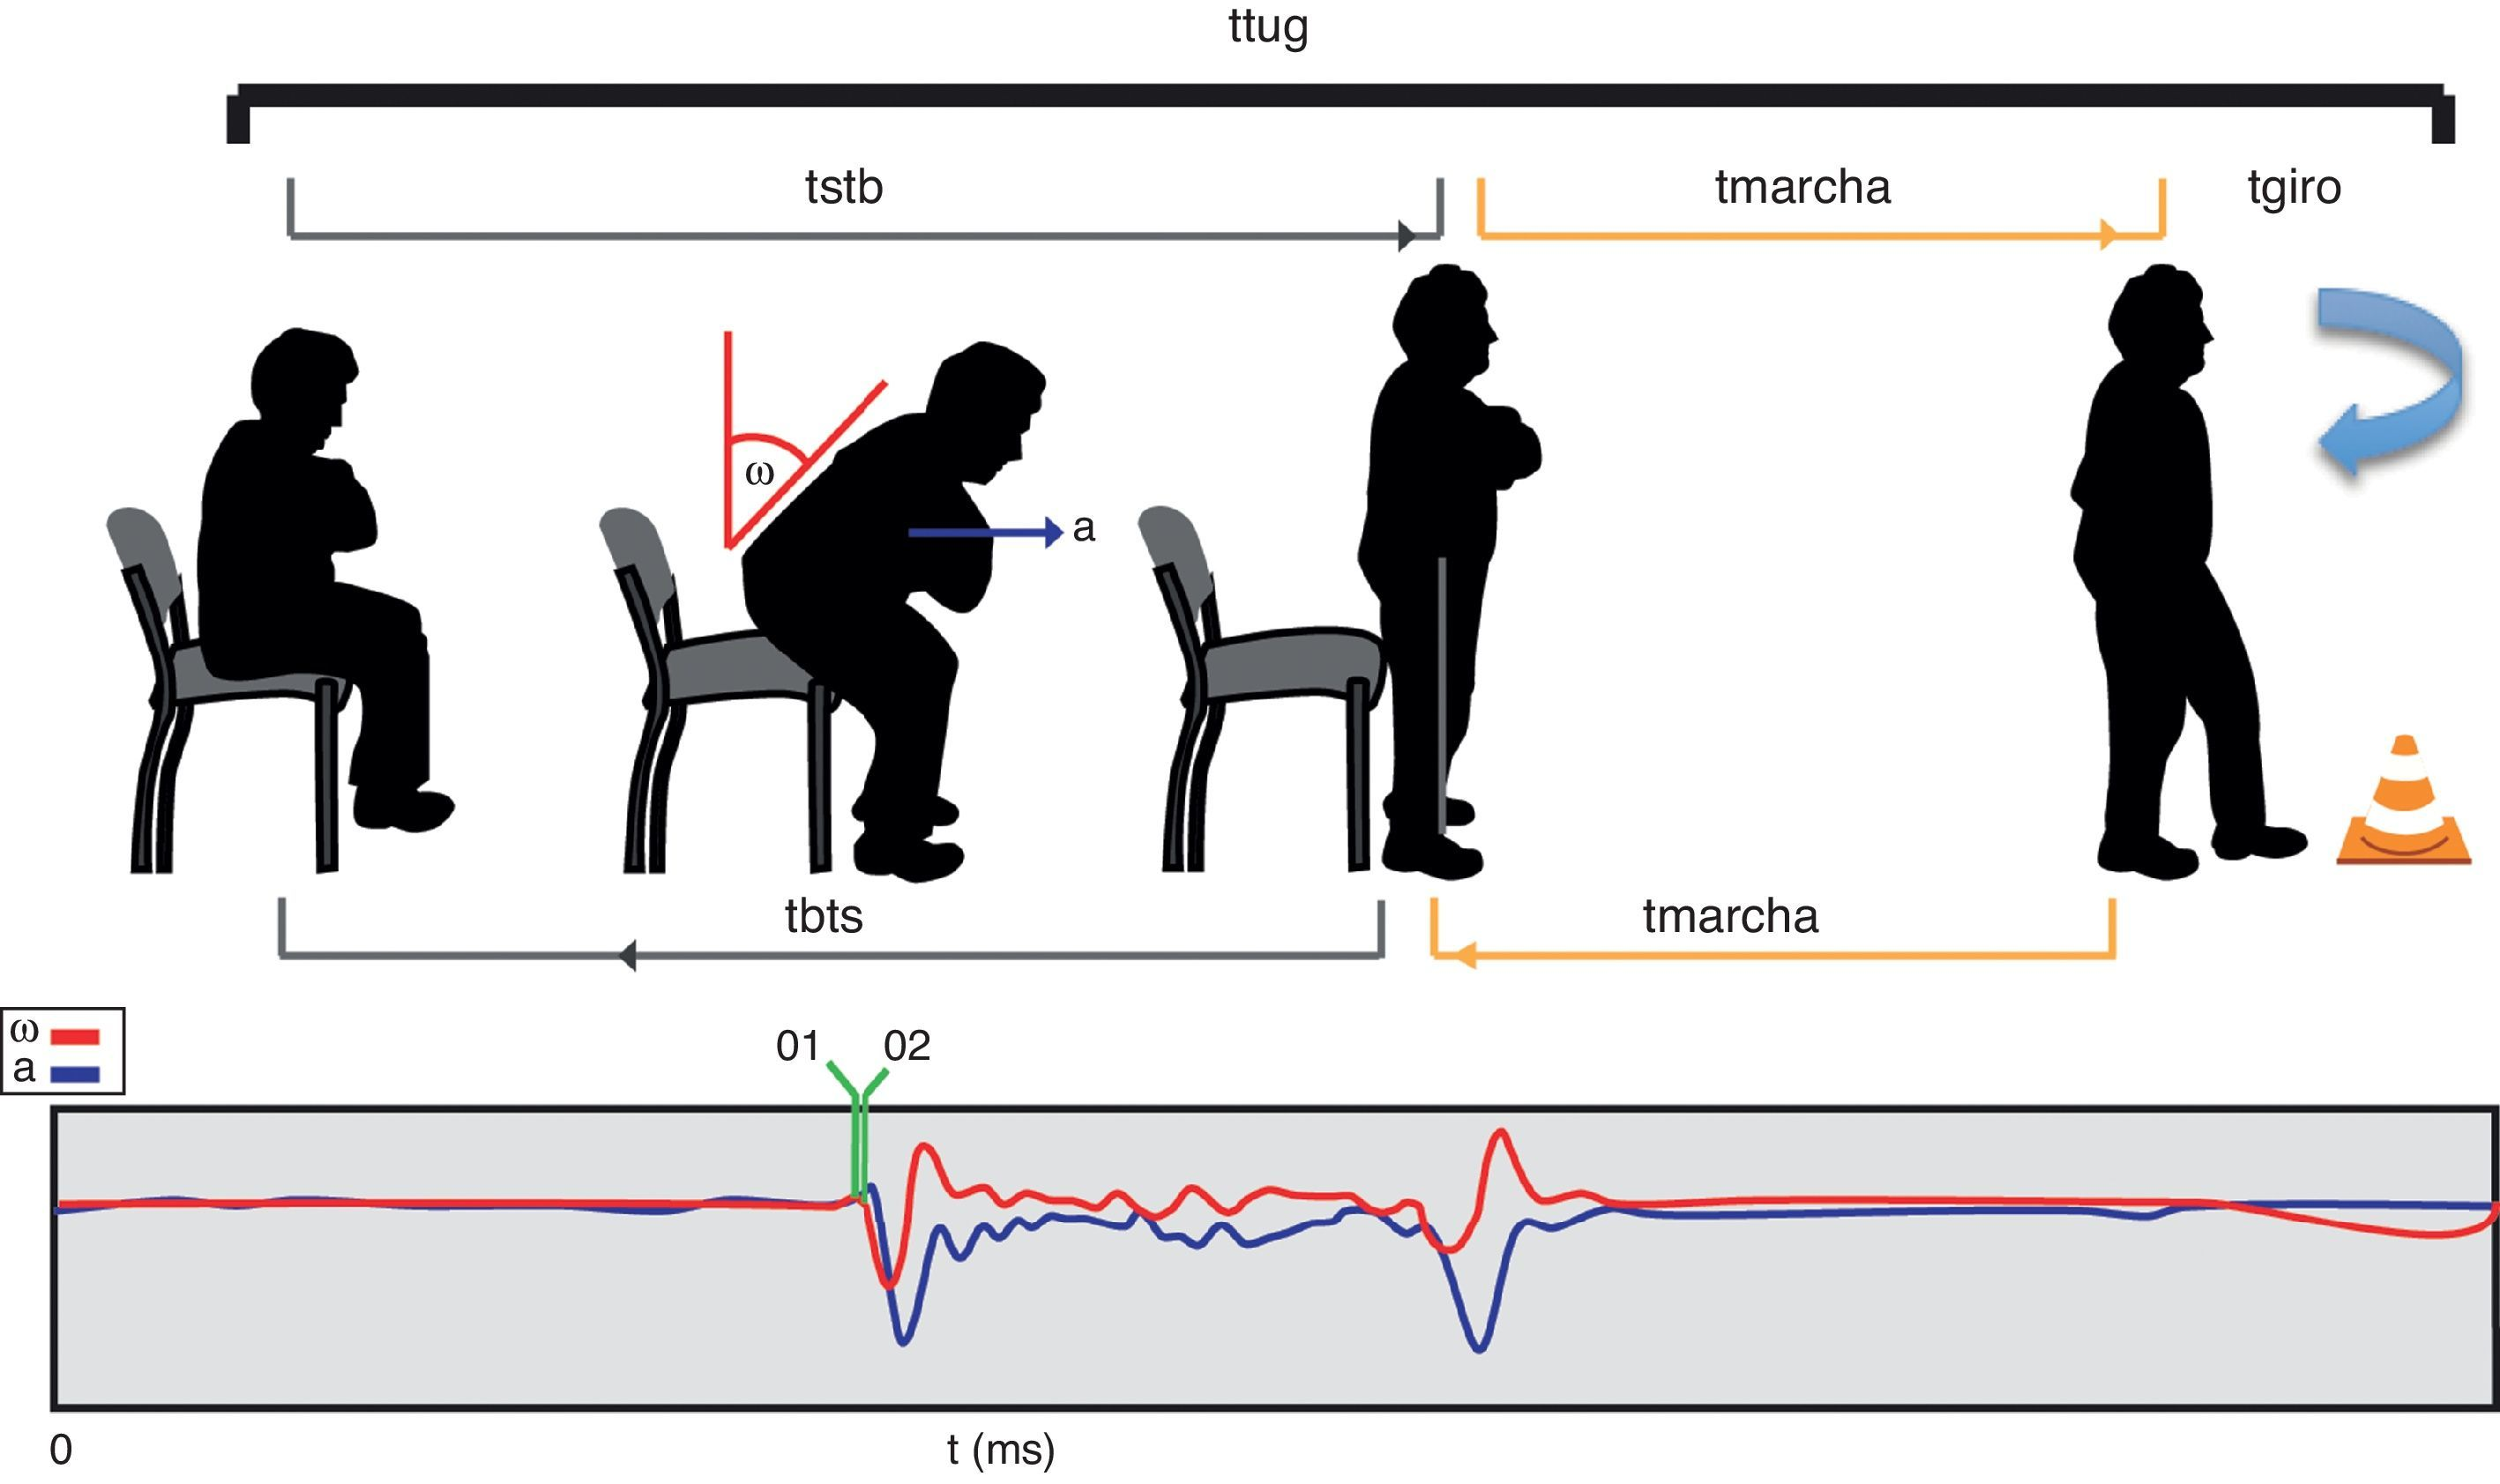
\includegraphics[width=\linewidth]{Images/TimedUpAndGoPhases.jpeg}
      {\tiny Señales de velocidad angular ($\omega$) y aceleración ($a$) del sensor lumbar durante las fases del TUG}
  \end{columns}
\end{frame}

% -------- DIAPOSITIVA 4: MOTIVACIÓN Y PROBLEMA --------
\begin{frame}{Motivación y Planteamiento del Problema}
  \begin{columns}[t]
    \column{0.48\textwidth}
      \begin{alertblock}{Limitaciones actuales}
        \begin{itemize}
          \item Sistemas iTUG comerciales: \textbf{costosos}, poco portátiles
          \item Trabajo previo (Pérez Kuleshova, 2021):\\
                prototipo sin gestión autónoma de pacientes, sin
                persistencia estructurada, sin integración a
                plataforma centralizada
        \end{itemize}
      \end{alertblock}
    \column{0.48\textwidth}
      \begin{block}{Oportunidad}
        Los smartphones integran sensores inerciales MEMS de
        alta disponibilidad y bajo costo.\\[0.5em]
        \textbf{¿Es posible} desarrollar un sistema autónomo,
        conectado y \textbf{clínicamente válido} usando el smartphone?
      \end{block}
      \vspace{0.5em}
      \begin{block}{Respuesta (este trabajo)}
        Sistema de tres capas: \textbf{app Android autoTUG} +
        \textbf{backend} + \textbf{plataforma de la marcha (GICI)}
        $\Rightarrow$ TRL~6
      \end{block}
  \end{columns}
\end{frame}

% -------- DIAPOSITIVA 5: OBJETIVOS --------
\begin{frame}{Objetivos}
  \begin{block}{Objetivo General}
    Desarrollar una aplicación móvil Android para la monitorización
    de la prueba TUG con gestión de información en la nube,
    alcanzando un nivel de madurez tecnológica \textbf{TRL~6}.
  \end{block}
  \vspace{0.6em}
  \textbf{Objetivos específicos:}
  \begin{enumerate}
    \item Implementar la adquisición a 50\,Hz, segmentación temporal y
          cálculo de variables biomecánicas mediante los sensores MEMS del
          smartphone
    \item Desarrollar los módulos de gestión de pacientes con modos
          \textit{offline} y \textit{online} (autenticación JWT)
    \item Integrar el microservicio TUG en la plataforma de la marcha
          del grupo GICI
    \item Validar el sistema frente al sensor inercial comercial
          BTS\,GSensor mediante ICC(2,1) y Bland--Altman
  \end{enumerate}
\end{frame}

% ============================================================
\section{Sistema Desarrollado}

% -------- DIAPOSITIVA 6: ARQUITECTURA --------
\begin{frame}{Arquitectura General del Sistema autoTUG}
  \centering
  \begin{tikzpicture}[node distance=0.65cm and 1.5cm]
    % Nodos
    \node[sblock, text width=2.6cm]             (sensor)   {\textbf{Sensores MEMS}\\\small Acelerómetro\\Giroscopio\\50\,Hz};
    \node[sblock, right=of sensor, text width=2.6cm] (app) {\textbf{App Android}\\\small autoTUG\\Kotlin};
    \node[sblock, right=of app, text width=2.6cm]   (srv)  {\textbf{Backend PHP}\\\small JWT Auth\\API REST};
    \node[sblock, right=of srv, text width=2.6cm]   (plat) {\textbf{Plataforma GICI}\\\small Microservicio\\TUG};
    \node[sblock, below=0.6cm of plat, text width=2.6cm, fill=lightgold]
                                                    (rep)  {\textbf{Informe}\\\small Variables\\biomecánicas};
    % Flechas
    \draw[sarrow] (sensor) -- (app);
    \draw[sarrow] (app) -- node[above,font=\tiny]{CSV + JWT} (srv);
    \draw[sarrow] (srv) -- node[above,font=\tiny]{procesa} (plat);
    \draw[sarrow] (plat) -- (rep);
    % Vuelta del informe
    \draw[sarrow] (rep.west) -- +(-0.5,0) -- +(- 0.5,-0.8)
                  -- node[below,font=\tiny]{informe al profesional} +(-9.5,-0.8)
                  -- +(-9.5,0.0) -- (app.south);
  \end{tikzpicture}
  \vspace{0.5em}

  \begin{columns}[c]
    \column{0.32\textwidth}
      \centering
      {\small\textbf{Capa 1}\\\textit{Adquisición y gestión}\\en el smartphone}
    \column{0.32\textwidth}
      \centering
      {\small\textbf{Capa 2}\\\textit{Autenticación y envío}\\servidor PHP}
    \column{0.32\textwidth}
      \centering
      {\small\textbf{Capa 3}\\\textit{Procesamiento y reporte}\\plataforma GICI}
  \end{columns}
\end{frame}

% -------- DIAPOSITIVA 7: APP ANDROID --------
\begin{frame}{Aplicación Android autoTUG}
  \begin{columns}[t]
    \column{0.52\textwidth}
      \textbf{Funcionalidades principales:}
      \begin{itemize}
        \item Gestión de pacientes y pruebas con persistencia local
              (SQLite)
        \item Modo \textit{offline}: funciona sin conexión,
              sincroniza automáticamente al reconectar
        \item Modo \textit{online}: autenticación JWT,
              envío cifrado al servidor
        \item Inicio y fin \textbf{automáticos} de la prueba
              (criterio de inactividad de 5\,s)
        \item Tutorial integrado — reduce errores operativos
        \item Lectura sonora de inicio y cierre de captura
      \end{itemize}
      \vspace{0.3em}
      {\small Desarrollada en \textbf{Kotlin} para Android}
    \column{0.45\textwidth}
      \centering
      \begin{subfigure}[b]{0.48\linewidth}
        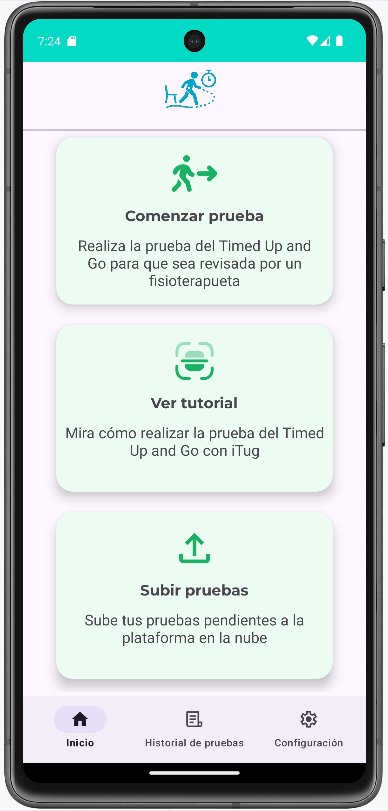
\includegraphics[width=\linewidth]{Images/HomeViewAutoTug.png}
      \end{subfigure}
      \hfill
      \begin{subfigure}[b]{0.48\linewidth}
        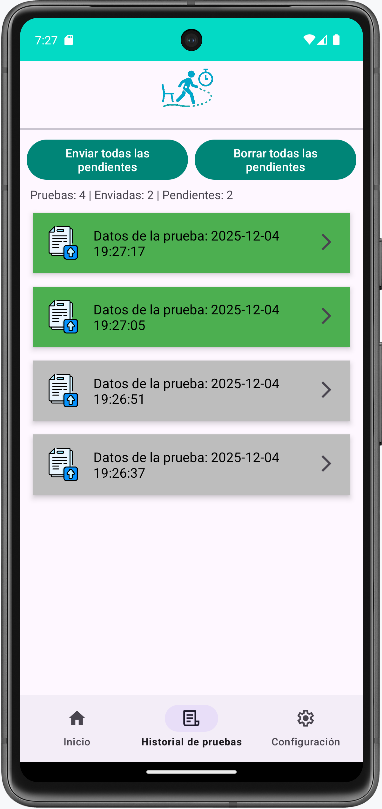
\includegraphics[width=\linewidth]{Images/HistorialPruebasAutoTug.png}
      \end{subfigure}\\[0.3em]
      \begin{subfigure}[b]{0.96\linewidth}
        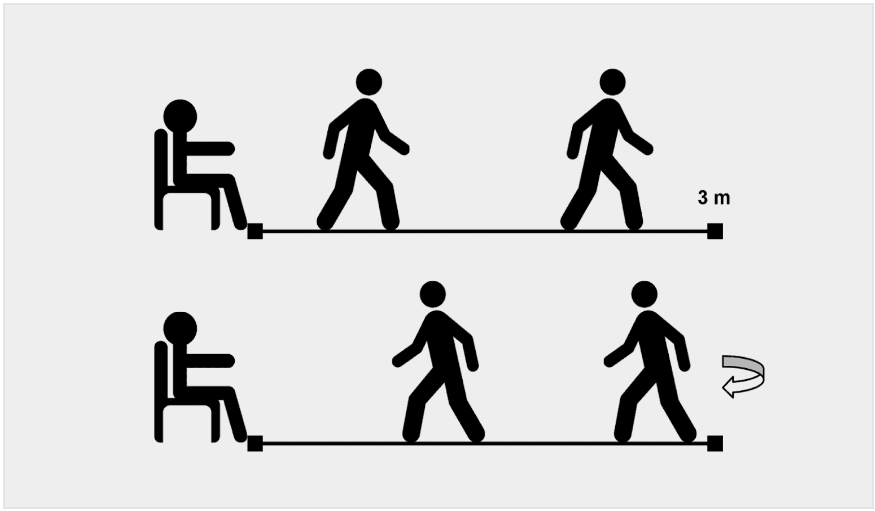
\includegraphics[width=\linewidth]{Images/TUG_Test.png}
      \end{subfigure}
      {\tiny Pantalla principal, historial y pantalla de prueba}
  \end{columns}
\end{frame}

% -------- DIAPOSITIVA 8: UBICACIÓN Y CALIBRACIÓN --------
\begin{frame}{Ubicación y Calibración del Dispositivo}
  \begin{columns}[t]
    \column{0.50\textwidth}
      \begin{block}{Ubicación: región lumbar L2}
        \begin{itemize}
          \item Cercanía al centro de masa del cuerpo
          \item Coherente con la ubicación del BTS\,GSensor
          \item Fijación con portacelular (riñonera horizontal)
        \end{itemize}
      \end{block}
      \vspace{0.5em}
      \begin{block}{Calibración: 3 referencias de señal}
        \begin{enumerate}
          \small
          \item \textbf{\textit{Zero-rate offset}} del giroscopio
                (3 ejes) — compensa el sesgo del sensor
          \item \textbf{Vector de gravedad} del acelerómetro —
                define el eje vertical (craneocaudal)
          \item \textbf{Offset de \textit{yaw}} — alinea las
                aceleraciones con los ejes clínicos AP / ML
        \end{enumerate}
        \vspace{0.2em}
        {\small Si la orientación es inadecuada, la app la solicita antes de
        iniciar la prueba.}
      \end{block}
    \column{0.47\textwidth}
      \centering
      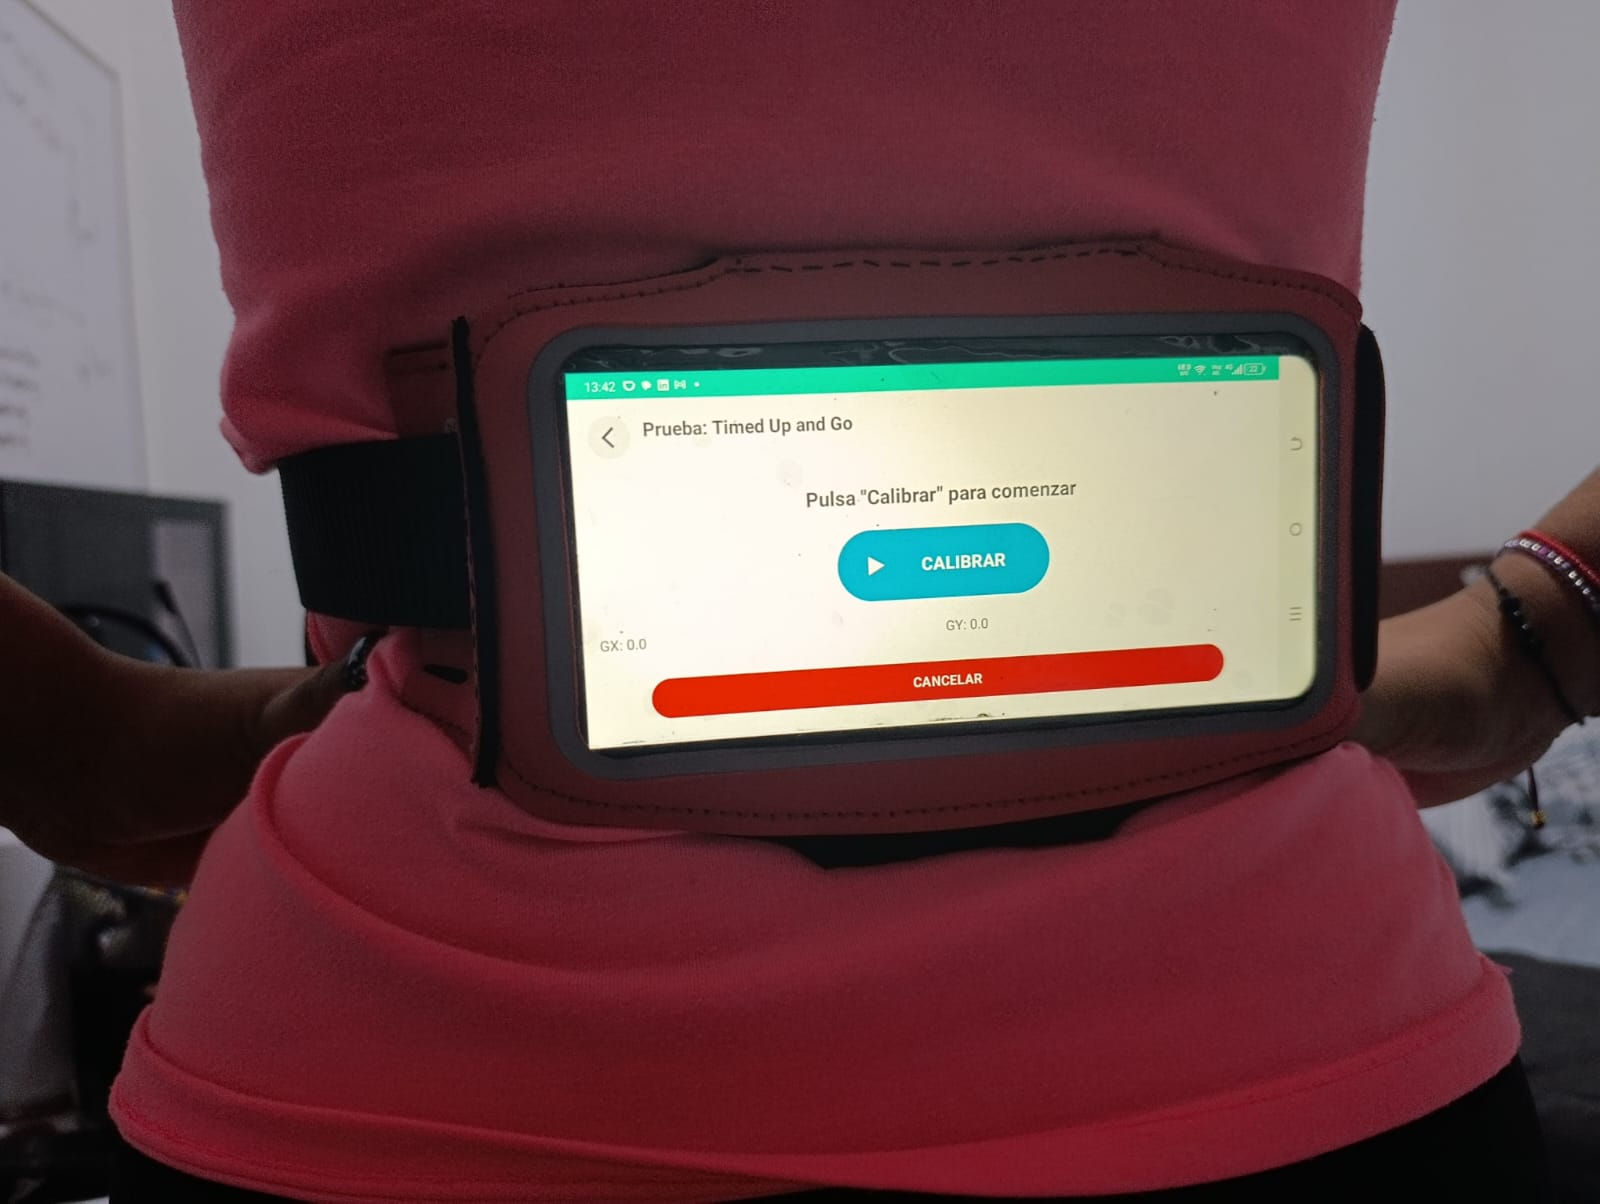
\includegraphics[width=0.80\linewidth]{Images/Cellphone_position_autoTug.jpeg}\\
      \vspace{0.4em}
      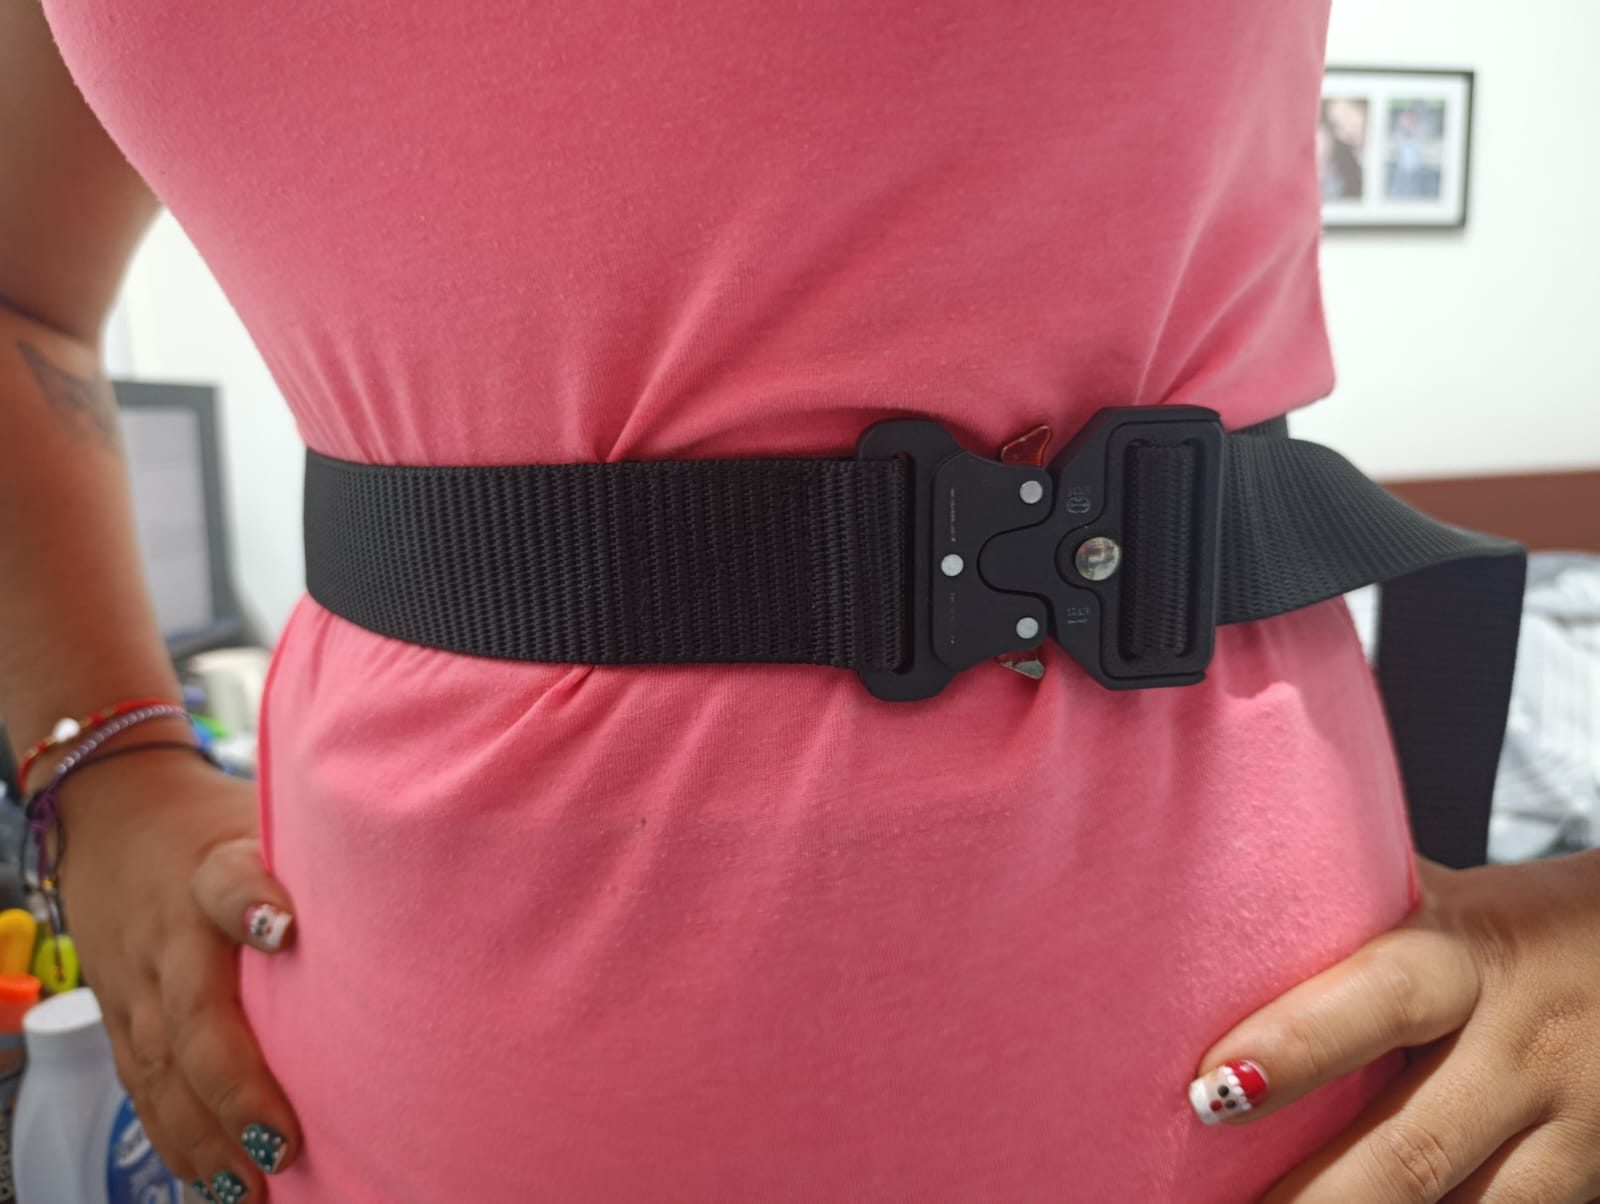
\includegraphics[width=0.80\linewidth]{Images/Belt_Cellphone.jpeg}
      {\tiny Montaje: BTS (abajo) + teléfono (arriba) en L2}
  \end{columns}
\end{frame}

% ============================================================
\section{Procesamiento de Señales}

% -------- DIAPOSITIVA 9: ADQUISICIÓN DIGITAL --------
\begin{frame}{Adquisición Digital: Sensores MEMS a 50\,Hz}
  \begin{columns}[c]
    \column{0.52\textwidth}
      \begin{block}{Características de adquisición}
        \begin{itemize}
          \item Sensores MEMS integrados en el teléfono
          \item Salida \textbf{digital directa} — sin ADC externo
          \item Frecuencia nominal: \alert{\textbf{50\,Hz}} (20\,ms/muestra)
          \item Cada muestra con \textit{timestamp} del SO
          \item $\Delta t_i$ \textbf{real} por par de muestras (Android
                no es determinista)
        \end{itemize}
      \end{block}
    \column{0.45\textwidth}
      \centering
      \begin{tabular}{lll}
        \toprule
        \textbf{Tipo} & \textbf{Señal} & \textbf{Unidad}\\
        \midrule
        \multirow{2}{*}{\small Física}
          & $a_x, a_y, a_z$ & m/s$^2$\\
          & $g_x, g_y, g_z$ & rad/s\\[3pt]
        \multirow{3}{*}{\small Indirecta}
          & $\theta_x, \theta_y$ & rad\\
          & roll, pitch, yaw & °\\
          & $a_{AP}, a_{ML}, a_{VT}$ & m/s$^2$\\
        \bottomrule
      \end{tabular}
      \vspace{0.5em}

      {\small \textbf{Físicas}: medidas directamente por el sensor MEMS\\[0.2em]
      \textbf{Indirectas}: calculadas por integración numérica o
      fusión de sensores}
  \end{columns}
\end{frame}

% -------- DIAPOSITIVA 10: EJES --------
\begin{frame}{Correspondencia: Ejes del Giroscopio vs. Ejes Anatómicos}
  \centering
  \begin{tabular}{llll}
    \toprule
    \textbf{Eje dispositivo} & \textbf{Señal}
      & \textbf{Plano anatómico / movimiento} & \textbf{Uso}\\
    \midrule
    X — lateral del teléfono  & $g_x$
      & Sagital — flexión/extensión del tronco & Transiciones posturales\\
    Y — longitudinal          & $g_y$
      & Transversal — giro corporal 180°       & Detección de giros\\
    Z — perp. a la pantalla   & $g_z$
      & Coronal — balanceo lateral             & No utilizado\\
    \bottomrule
  \end{tabular}

  \vspace{0.6em}
  \begin{columns}[c]
    \column{0.55\textwidth}
      \begin{block}{Robustez por software (auto-swap)}
        Se comparan los rangos integrados:
        $R_x = \max(\theta_x)-\min(\theta_x)$,\;
        $R_y = \max(\theta_y)-\min(\theta_y)$\\[0.3em]
        Si $R_y < 0.5\,R_x \Rightarrow$ intercambio automático
        $g_x \leftrightarrow g_y$\\[0.2em]
        La asignación es \textbf{correcta independientemente}
        de cómo quede orientado el teléfono en el portacelular.
      \end{block}
    \column{0.42\textwidth}
      \centering
      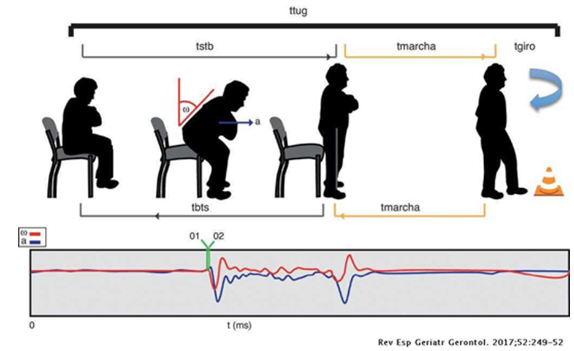
\includegraphics[width=0.88\linewidth]{Images/Esquema_susFases_TUG.png}
      {\tiny Ejes de referencia y subfases del TUG}
  \end{columns}
\end{frame}

% -------- DIAPOSITIVA 11: ALGORITMO SEGMENTACIÓN --------
\begin{frame}{Algoritmo de Segmentación Temporal}
  \begin{columns}[t]
    \column{0.52\textwidth}
      \begin{block}{Idea central}
        \textbf{Medición indirecta:}
        $\theta_x(t) = \int g_x\,dt$,\;\;
        $\theta_y(t) = \int g_y\,dt$\\[0.4em]
        Una transición postural o un giro generan
        \textbf{acumulación sostenida} en $\theta$;
        el ruido durante la marcha no la alcanza.
      \end{block}
      \vspace{0.4em}
      \textbf{Reglas determinísticas:}
      \begin{itemize}
        \small
        \item $g_x > 0.1$\,rad/s \textbf{y} $\theta_x > 0.1$\,rad
              $\Rightarrow$ inicio sentado--parado
        \item $|\theta_y| > 0.9$\,rad (umbral externo) con búsqueda
              retro\-activa a 0.6\,rad $\Rightarrow$ inicio giro~1
        \item Ventana de 10 muestras con $g_y = 0$
              $\Rightarrow$ fin giro~1 / inicio marcha~2
        \item Tendencia $|\dot\theta_y| > 0.5$\,rad/s
              + umbrales de confirmación $\Rightarrow$ giro~2
      \end{itemize}
      \vspace{0.2em}
      {\small Umbrales ajustados \textbf{empíricamente} sobre datos propios (L2, 50\,Hz)}
    \column{0.45\textwidth}
      \centering
      %% *** IMAGEN: convertir a PNG desde SVG ***
      %% Velocity_Angular_Position_Signals_1.svg  (Fig 4.1 del documento)
      \fbox{\parbox{0.92\linewidth}{%
        \centering\vspace{2.2cm}
        \small [Señales $g_y$ y $\theta_y$ durante el TUG\\
        — Fig.~4.1 del documento —\\
        \textit{(exportar SVG a PNG)}]
        \vspace{2.2cm}}}
      {\tiny Acumulación en $\theta_y$ discrimina giros reales de derivas durante la marcha}
  \end{columns}
\end{frame}

% -------- DIAPOSITIVA 12: EFECTO DEL CONO --------
\begin{frame}{Robustez ante Variaciones de Trayectoria}
  \begin{columns}[c]
    \column{0.48\textwidth}
      \centering
      %% *** Velocity_Angular_Position_Signals_1.svg → PNG ***
      \fbox{\parbox{0.92\linewidth}{%
        \centering\vspace{2.0cm}
        \small [Prueba \textbf{sin cono}\\
        Giro abrupto sobre el propio eje\\
        — Fig.~4.1 —]
        \vspace{2.0cm}}}
      {\tiny Giro \textbf{abrupto}: $\theta_y$ crece rápidamente}
    \column{0.48\textwidth}
      \centering
      %% *** Velocity_Angular_Position_Signals_2.svg → PNG ***
      \fbox{\parbox{0.92\linewidth}{%
        \centering\vspace{2.0cm}
        \small [Prueba \textbf{con cono}\\
        Pico previo negativo en $g_y$\\
        por ajuste de trayectoria\\
        — Fig.~4.2 —]
        \vspace{2.0cm}}}
      {\tiny Pico previo en $g_y$ por rodear el cono; el doble umbral lo absorbe}
  \end{columns}
  \vspace{0.4em}
  \begin{center}
    {\small El doble umbral externo/interno en $\theta_y$
    (0.9\,/\,0.6\,rad) hace el detector \textbf{robusto al estilo de giro}}
  \end{center}
\end{frame}

% -------- DIAPOSITIVA 13: VARIABLES BIOMECÁNICAS --------
\begin{frame}{Transformación de Marco y Variables Biomecánicas}
  \begin{columns}[c]
    \column{0.42\textwidth}
      \centering
      \begin{tikzpicture}[node distance=0.22cm, scale=0.80, transform shape]
        \node[sblock, text width=3.6cm]                (a){Marco dispositivo\\$(a_x,a_y,a_z)$};
        \node[sblock, below=of a, text width=3.6cm]    (b){Rotación Euler Z--Y--X\\(yaw--pitch--roll)};
        \node[sblock, below=of b, text width=3.6cm]    (c){Compensación gravedad\\$-9{,}81$\,m/s$^2$};
        \node[sblock, below=of c, text width=3.6cm]    (d){Filtro pasa--bajo\\$f_c = 9$\,Hz \textit{(fwd-bwd)}};
        \node[sblock, below=of d, text width=3.6cm]    (e){Offset de \textit{yaw}\\(promedio 3\,s reposo)};
        \node[sblock, below=of e, text width=3.6cm,
              fill=lightgold]                           (f){$a_{AP},\;a_{ML},\;a_{VT}$\\Ejes clínicos};
        \foreach \i/\j in {a/b,b/c,c/d,d/e,e/f}
          \draw[sarrow] (\i) -- (\j);
      \end{tikzpicture}
    \column{0.55\textwidth}
      \textbf{Variables calculadas por subfase:}\\[0.3em]
      \begin{tabular}{ll}
        $t_{stb}, t_{g1}, t_{turn1}, \ldots$ & Tiempos por subfase\\[2pt]
        $\Delta a_{AP}, \Delta a_{ML}, \Delta a_{VT}$ & Rangos pico--a--pico\\[2pt]
        $|g_y|_{max},\;|g_y|_{mean}$ & Velocidad angular de giro\\[2pt]
        $\theta_{flex},\;\theta_{ext}$ & Flexión/extensión tronco\\[2pt]
      \end{tabular}
      \vspace{0.5em}
      \begin{block}{Microservicio TUG (PHP)}
        Recibe el CSV del sensor, ejecuta toda la cadena de procesamiento
        de forma automática y devuelve el informe con las variables
        a la plataforma GICI.
      \end{block}
  \end{columns}
\end{frame}

% -------- DIAPOSITIVA 14: PLATAFORMA GICI --------
\begin{frame}{Plataforma de la Marcha Humana — GICI}
  \begin{columns}[c]
    \column{0.47\textwidth}
      \centering
      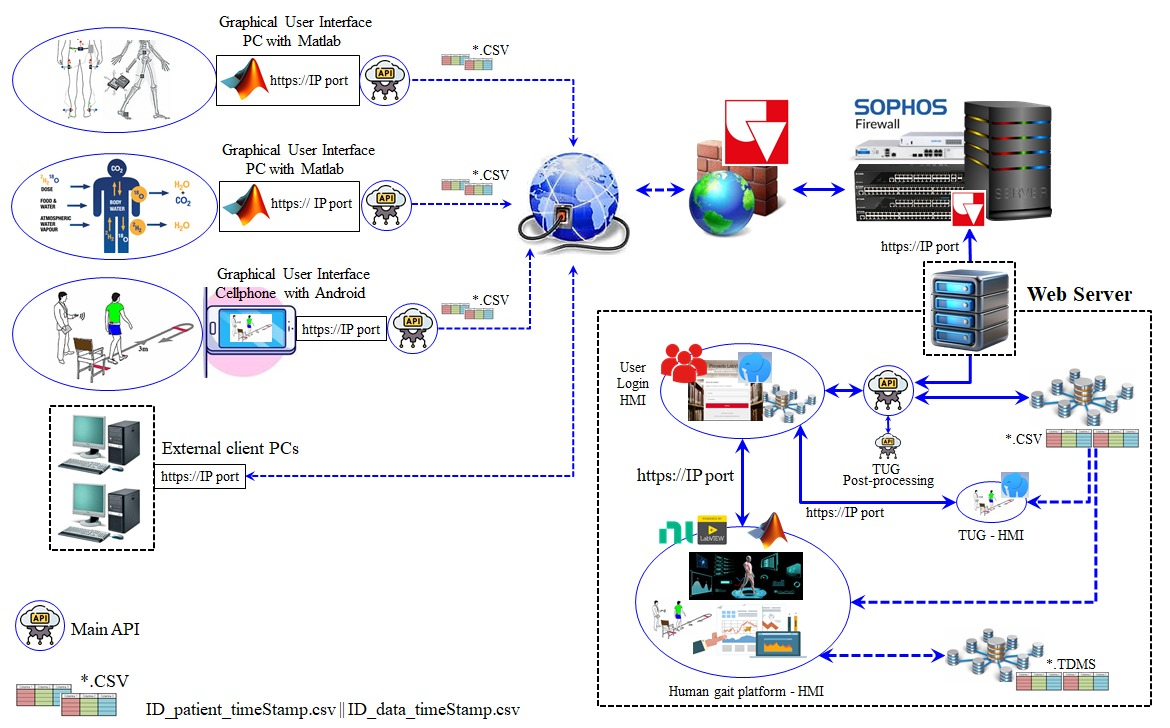
\includegraphics[width=\linewidth]{Images/Gait_Platform_Infrastructure.jpeg}
      {\tiny Arquitectura cliente--servidor de la plataforma}
    \column{0.50\textwidth}
      \centering
      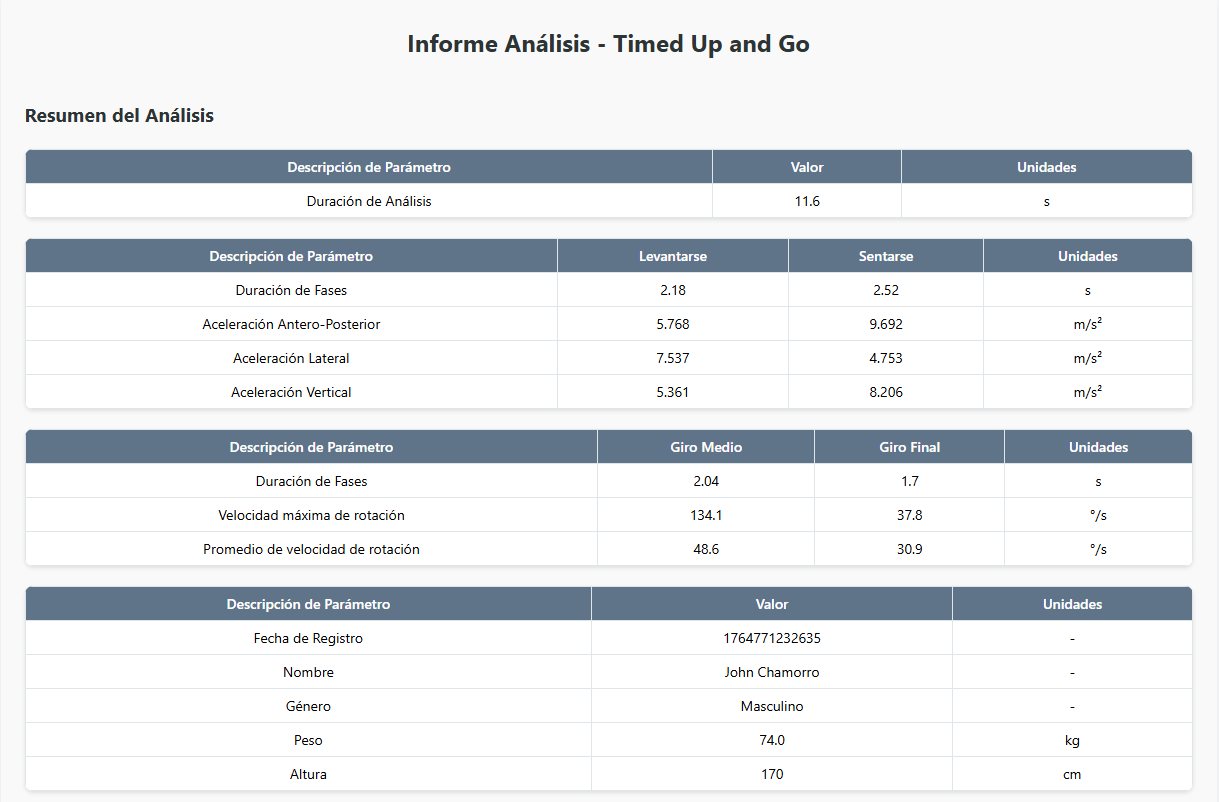
\includegraphics[width=\linewidth]{Images/Analysis_report_1.png}\\[0.25em]
      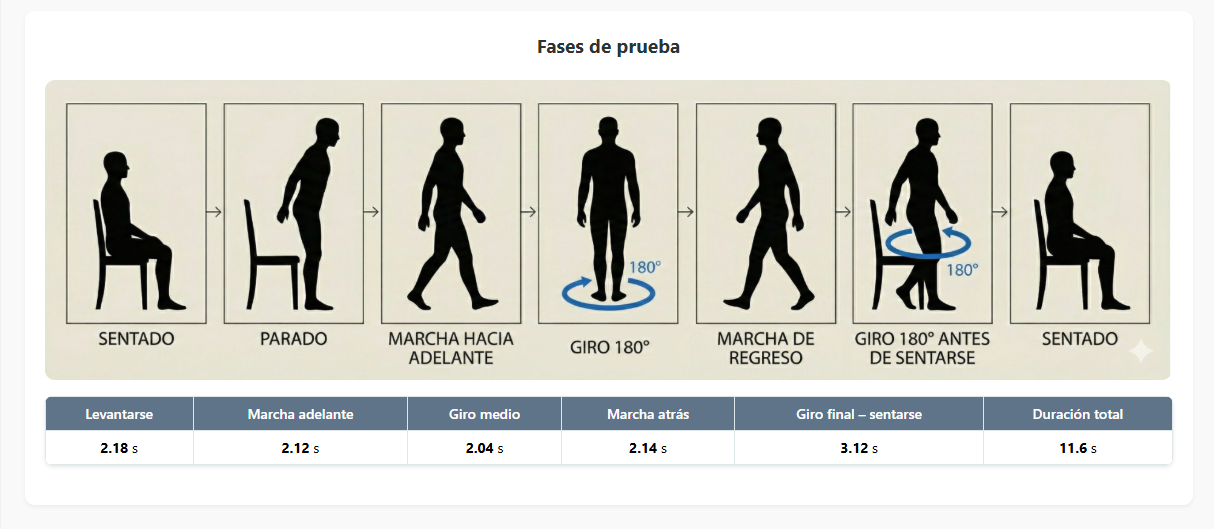
\includegraphics[width=\linewidth]{Images/Analysis_report_2.png}
      {\tiny Informe: variables biomecánicas (arriba) y tiempos de subfases (abajo)}
  \end{columns}
\end{frame}

% ============================================================
\section{Validación Experimental}

% -------- DIAPOSITIVA 15: PROTOCOLO --------
\begin{frame}{Protocolo de Validación}
  \begin{columns}[t]
    \column{0.50\textwidth}
      \begin{block}{Configuración experimental}
        \begin{itemize}
          \item Laboratorio SERH, Universidad del Valle
          \item \textbf{7 sujetos, 14 ensayos} — adultos sanos
          \item Protocolo de bajo riesgo (aval Comité de Ética UV)
          \item \textbf{BTS\,GSensor}: referencia clínica práctica
                (no \textit{gold standard}; algoritmo de segmentación
                 \textbf{propietario})
        \end{itemize}
      \end{block}
      \vspace{0.4em}
      \textbf{Montaje simultáneo en L2:}\\
      \hspace{0.5em}$\blacktriangleright$ BTS fijo al portacelular\\
      \hspace{0.5em}$\blacktriangleright$ Teléfono encima del BTS\\
      \hspace{0.5em}$\blacktriangleright$ Ambos comparten el movimiento\\[0.3em]
      {\small Diferencias de muestreo: BTS 100\,Hz vs.\ app 50\,Hz}\\
      {\small \textit{Offset} espacial $\delta$ entre sensores}
    \column{0.47\textwidth}
      \centering
      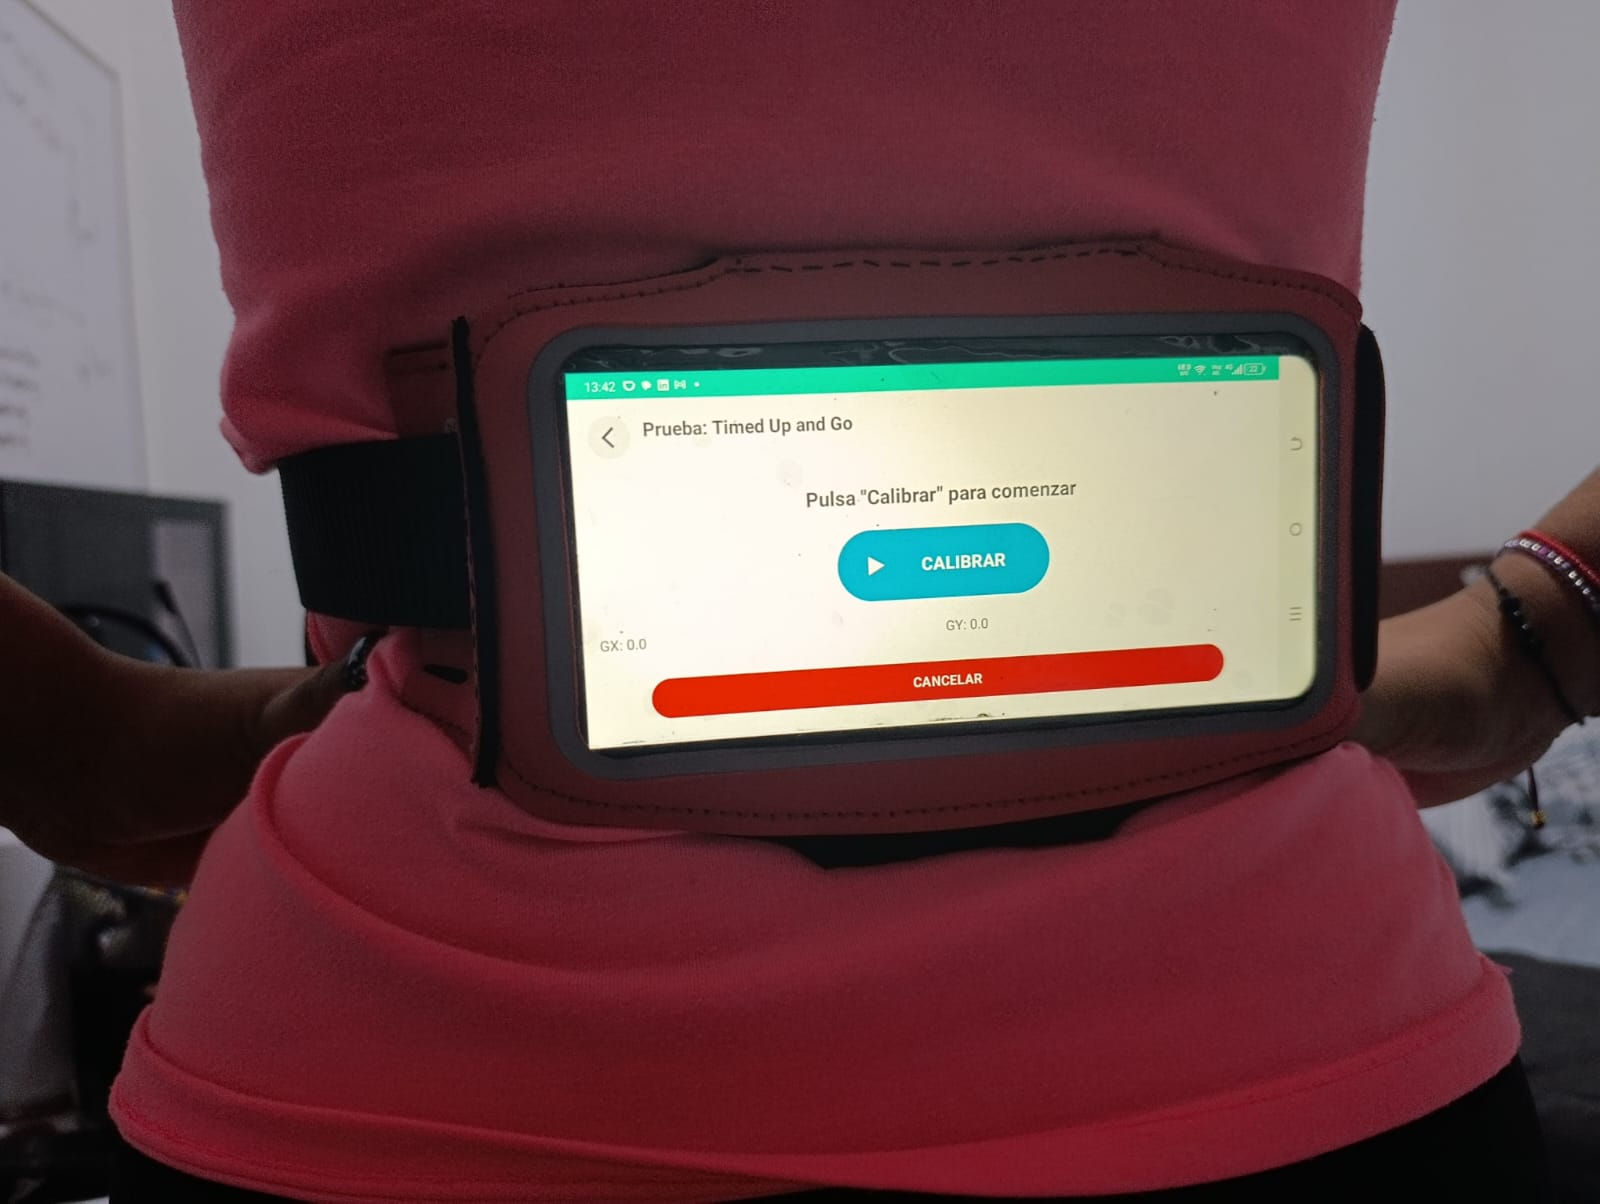
\includegraphics[width=0.82\linewidth]{Images/Cellphone_position_autoTug.jpeg}\\
      \vspace{0.5em}
      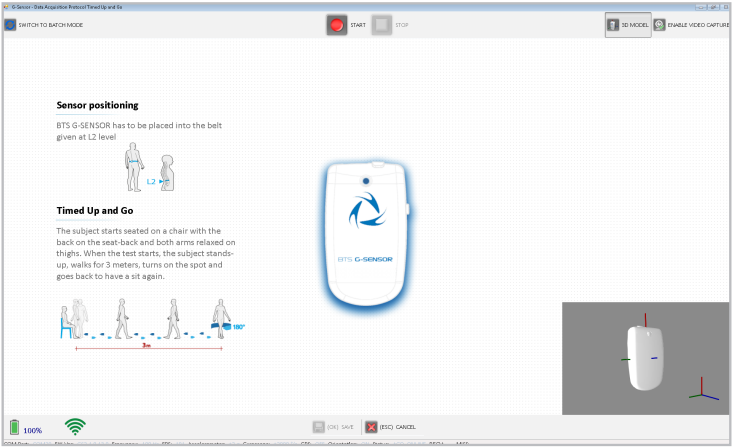
\includegraphics[width=0.82\linewidth]{Images/TUG_BTS_RecordingScreen.png}
      {\tiny Arriba: montaje en L2. Abajo: pantalla del BTS durante el ensayo}
  \end{columns}
\end{frame}

% -------- DIAPOSITIVA 16: RESULTADOS — TIEMPO TOTAL --------
\begin{frame}{Resultados: Tiempo Total del TUG}
  \begin{columns}[c]
    \column{0.48\textwidth}
      \centering
      \small
      \begin{tabular}{lc}
        \toprule
        \textbf{Métrica (tiempo total)} & \textbf{Valor}\\
        \midrule
        Sesgo (s)             & $+0{,}186$\\
        SD$_\text{diff}$ (s)  & $0{,}193$\\
        MAE (s)               & $0{,}239$\\
        RMSE (s)              & $0{,}263$\\
        LoA$_\text{low}$ (s)  & $-0{,}192$\\
        LoA$_\text{high}$ (s) & $+0{,}565$\\
        MAPE (\%)             & $2{,}02$\\
        \midrule
        \textbf{ICC(2,1)}     & $\mathbf{0{,}994}$\\
        IC\,95\%              & $[0{,}94;\;1{,}00]$\\
        Interpretación        & \textcolor{green!55!black}{\textbf{Excelente}}\\
        \bottomrule
      \end{tabular}
      \vspace{0.4em}

      \begin{alertblock}{\small Aceptabilidad clínica}
        \small MDC clínico reportado: 2--3\,s\\
        LoA observados: $\leq 0{,}565$\,s\\
        $\Rightarrow$ \textbf{clínicamente aceptable}
      \end{alertblock}
    \column{0.49\textwidth}
      \centering
      %% *** Gráfico Bland-Altman del tiempo total ***
      %% Generar en R o Python y exportar como PNG/PDF
      \fbox{\parbox{0.94\linewidth}{%
        \centering\vspace{3.2cm}
        \textbf{[Gráfico Bland--Altman]}\\[0.3em]
        \small Tiempo total del TUG\\
        (n = 14 ensayos)\\[0.3em]
        Eje X: media de métodos (s)\\
        Eje Y: diferencia app$-$BTS (s)\\[0.3em]
        \textit{Insertar figura del análisis estadístico}
        \vspace{3.2cm}}}
  \end{columns}
\end{frame}

% -------- DIAPOSITIVA 17: RESULTADOS — SUBFASES --------
\begin{frame}{Resultados: Confiabilidad por Subfase (ICC)}
  \begin{columns}[t]
    \column{0.50\textwidth}
      \centering
      \small
      \begin{tabular}{lcc}
        \toprule
        \textbf{Subfase} & \textbf{ICC(2,1)}
          & \textbf{Interpretación}\\
        \midrule
        Sit-to-Stand  & 0{,}373 & Baja\\
        Gait 1        & 0{,}925 & \textcolor{green!55!black}{Excelente}\\
        Turn 1        & 0{,}604 & Moderada\\
        Gait 2        & 0{,}767 & Buena\\
        Turn 2        & 0{,}393 & Baja\\
        Stand-to-Sit  & 0{,}455 & Baja\\
        \midrule
        \textbf{Total}& \textbf{0{,}994}
          & \textcolor{green!55!black}{\textbf{Excelente}}\\
        \bottomrule
      \end{tabular}
    \column{0.47\textwidth}
      \begin{alertblock}{¿Por qué variabilidad en subfases?}
        \begin{enumerate}
          \small
          \item Eventos \textbf{cortos}: pequeñas diferencias
                absolutas $\to$ MAPE alto
          \item Criterios de inicio/fin \textbf{distintos}\\
                (BTS: algoritmo propietario)
          \item \textit{Offset} espacial $\delta$ entre sensores
          \item Diferencia de muestreo (100\,Hz vs.\,50\,Hz)
        \end{enumerate}
      \end{alertblock}
      \vspace{0.4em}
      {\small La discrepancia en subfases \textbf{no implica necesariamente
      error} del sistema desarrollado; puede reflejar
      \textbf{criterios de segmentación distintos}.}
  \end{columns}
\end{frame}

% ============================================================
\section{Conclusiones}

% -------- DIAPOSITIVA 18: TRL 6 --------
\begin{frame}{Nivel de Madurez Tecnológica TRL~6}
  \begin{columns}[c]
    \column{0.52\textwidth}
      \begin{block}{¿Qué es TRL~6?}
        \textbf{Prototipo funcional} validado en un
        \textbf{entorno relevante}: pruebas en condiciones cercanas
        al uso real.
      \end{block}
      \vspace{0.5em}
      \textbf{Evidencias que sustentan TRL~6:}
      \begin{itemize}
        \item Prototipo integrado (app + backend + microservicio)
        \item Ensayos en laboratorio SERH con sujetos reales
        \item Protocolo controlado con referencia clínica comercial
        \item ICC(2,1) $\approx 0{,}994$ para el tiempo total
        \item Informes automáticos generados y accesibles en la
              plataforma GICI
      \end{itemize}
    \column{0.45\textwidth}
      \centering
      %% *** Diagrama escala TRL 1-9 con nivel 6 resaltado ***
      %% (crear o insertar imagen)
      \fbox{\parbox{0.92\linewidth}{%
        \centering\vspace{3.8cm}
        \textbf{[Escala TRL 1--9]}\\[0.3em]
        \small con nivel 6 resaltado\\
        \textit{(insertar imagen)}
        \vspace{3.8cm}}}
  \end{columns}
\end{frame}

% -------- DIAPOSITIVA 19: CONCLUSIONES --------
\begin{frame}{Conclusiones}
  \begin{enumerate}
    \setlength{\itemsep}{0.55em}
    \item \textbf{Sistema autónomo e integrado:} la aplicación
          Android autoTUG, el backend JWT y el microservicio PHP
          conforman una solución funcional de tres capas para la
          monitorización del TUG.

    \item \textbf{Alta confiabilidad para el tiempo total:}
          ICC$(2,1) = 0{,}994$ y LoA $\ll$ MDC clínico respaldan el
          uso del sistema para el desenlace global.

    \item \textbf{Segmentación robusta:} el doble umbral y la
          verificación de orientación mejoran el trabajo previo y
          operan de forma completamente autónoma.

    \item \textbf{Integración en plataforma GICI:} el microservicio
          TUG genera informes automáticos con variables biomecánicas
          y tiempos de subfases accesibles por \textit{web}.

    \item \textbf{TRL~6 alcanzado:} prototipo validado en
          laboratorio con protocolo controlado y sujetos reales,
          consistente con la definición del nivel.
  \end{enumerate}
\end{frame}

% -------- DIAPOSITIVA 20: TRABAJOS FUTUROS --------
\begin{frame}{Trabajos Futuros}
  \begin{enumerate}
    \setlength{\itemsep}{0.6em}
    \item \textbf{Optimización de segmentación:} ventanas
          adaptativas, detección supervisada con anotaciones
          clínicas, algoritmos robustos a variabilidad inter-sujeto

    \item \textbf{Validación con población clínica:} adultos
          mayores, pacientes con Parkinson, ECV, fragilidad; tamaños
          muestrales suficientes para sub-análisis por grupo

    \item \textbf{Estandarización de variables adicionales:}
          protocolo de equivalencia de ejes, filtros y definiciones
          para comparabilidad con múltiples IMUs comerciales

    \item \textbf{Evolución de la plataforma:} reportes
          longitudinales, visualización avanzada, control de roles
          granular, exportación para investigación clínica
  \end{enumerate}
\end{frame}

% -------- DIAPOSITIVA 21: GRACIAS / PREGUNTAS --------
\begin{frame}[plain]
  \centering
  \vspace{0.8cm}
  {\Large\bfseries\color{uvblue} ¡Muchas gracias!}
  \vspace{0.8cm}

  \begin{columns}[c]
    \column{0.60\textwidth}
      \centering
      {\large John Sebastian Chamorro Narváez}\\[0.6em]
      {\small Ingeniería Electrónica\\
      Universidad del Valle — GICI\\[0.5em]
      Directores:\\
      Dr.-Ing. Esteban Rosero\\
      José Miguel Ramírez Scarpetta, Ph.D.}
    \column{0.35\textwidth}
      \centering
      
\includegraphics[width=0.65\linewidth]{Images/LogoUnivalle.jpg}
  \end{columns}

  \vspace{1.0cm}
  {\Large\bfseries\color{uvblue} ¿Preguntas?}
\end{frame}

\end{document}
